\section{Model Optimization}

\begin{frame}
\frametitle{Mobile Robot Navigation}
\textcolor{tudblue}{\textbf{Goal:}} Move robot to area while minimizing traveled distance
\vfill

\begin{columns}[T]
\begin{column}{0.6\textwidth}
MDP Model $\mathcal{M}$ should define:
\begin{itemize}
	\item Attainable states, corresponding to locations
	\item Possible actions, robot translations
\end{itemize}
\end{column}

\begin{column}{0.4\textwidth}
	
\end{column}

\end{columns}

\end{frame}

\begin{frame}
\frametitle{Model-Learning for Mobile Robot Navigation}

\begin{columns}[T]
\begin{column}{0.6\textwidth}
\begin{itemize}
	\item \textbf{TODO}
	\item[] 
	\item Simulation in Morse with a Scitos A5 robot
\end{itemize}
\end{column}
\begin{column}{0.5\textwidth}
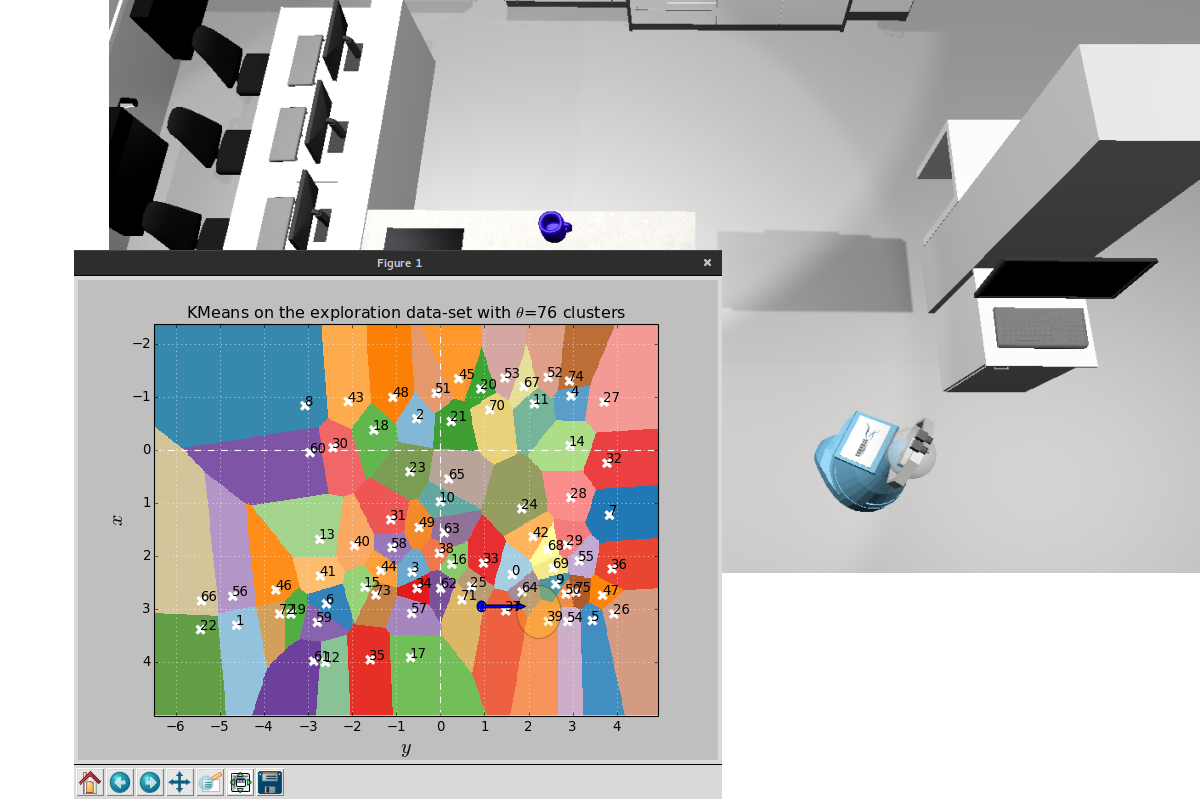
\includegraphics[width=\textwidth, left]{figures/simulation_learn_2}
\end{column}
\end{columns}	
	
\end{frame}

\begin{frame}
\frametitle{Model-Optimization Routine}
\begin{center}
\includegraphics<1| handout:0>[width=1\textwidth]{figures/optimization-routine/learning-cycle-1.pdf}
\includegraphics<2| handout:0>[width=1\textwidth]{figures/optimization-routine/learning-cycle-2.pdf}
\includegraphics<3| handout:0>[width=1\textwidth]{figures/optimization-routine/learning-cycle-3.pdf}
\includegraphics<4| handout:0>[width=1\textwidth]{figures/optimization-routine/learning-cycle-4.pdf}
\includegraphics<5>[width=1\textwidth]{figures/optimization-routine/learning-cycle-5.pdf}
\end{center}
\end{frame}

\begin{frame}
\frametitle{Model-Optimization Routine}
\begin{center}
	\includegraphics<1| handout:0>[width=1\textwidth]{figures/optimization-routine/learning-cycle-simplified-1.pdf}
	\includegraphics<2| handout:0>[width=1\textwidth]{figures/optimization-routine/learning-cycle-simplified-2.pdf}
	\includegraphics<3>[width=1\textwidth]{figures/optimization-routine/learning-cycle-simplified-3.pdf}
\end{center}
\end{frame}